\documentclass[10pt]{article}
\usepackage{geometry}
\geometry{a4paper, margin=1in}
\usepackage{graphicx}
\usepackage{amsmath, amssymb}
\usepackage{setspace}
\usepackage{titlesec}
\usepackage{fancyhdr}
\usepackage{hyperref}
\usepackage{listings}
\usepackage{xcolor}
\usepackage{enumitem}
\usepackage{fontspec}
\usepackage{subcaption}
\setmainfont{Times New Roman}

\titleformat{\section}{\large\bfseries}{\thesection.}{1em}{}
\titleformat{\subsection}{\normalsize\bfseries}{\thesubsection.}{1em}{}

\pagestyle{fancy}
\fancyhf{}
\rhead{Luna Sugiyama}
\lhead{Wed2 Natural Language Processing}
\rfoot{\thepage}

\title{\textbf{Final Report:\\Evaluation of Various Software Development AI Assistants}}
% \vspace{0.5em}
% \large [Optional Subtitle]}
\author{
    \makebox[\textwidth][c]{\textbf{Luna Sugiyama}} \\
    \makebox[\textwidth][c]{Graduate School of Information Science and Technology} \\
    \makebox[\textwidth][c]{Information and Communication Engineering} \\
    \makebox[\textwidth][c]{\texttt{lunagracesugiyama@g.ecc.u-tokyo.ac.jp}}
}
\date{\today}

\begin{document}

\maketitle
\thispagestyle{fancy}
I have recently been interested in Claude Code, and Gemini CLI which are AI assistant tools to help software development~\cite{vibecoding}.
However, due to the pricing I have not been able to use them extensively.
I thought this would be a good opportunity to explore these tools.
In this report I will choose these services and evaluate them on various tasks and aspects to see their strengths and weaknesses.

\section{About Each Service}
\subsection{Claude Code}
Claude Code is a code-centric variant of the Claude family of AI models developed by Anthropic. It is optimized for software development and programming-related tasks, such as code generation, debugging, explanation, and refactoring. Built on Anthropic's principles of Constitutional AI, Claude Code emphasizes helpfulness, honesty, and harmlessness while engaging in code-focused dialogues.
Claude Code can understand complex software engineering contexts and generate or edit code in a variety of programming languages including Python, JavaScript, TypeScript, and more. It supports in-depth reasoning about existing codebases and integrates well into workflows via the Claude API or the Claude web interface.
Key features of Claude Code include:
\begin{itemize}
    \item \textbf{Code Generation:} Generates new code snippets based on natural language
    \item \textbf{Debugging:} Identifies and fixes bugs in existing code
    \item \textbf{Code Explanation:} Provides explanations for code snippets, including complex algorithms
    \item \textbf{Refactoring:} Suggests improvements to existing code for better performance or readability
    \item \textbf{Multi-language Support:} Works with multiple programming languages
    \item \textbf{Contextual Understanding:} Maintains context across multiple interactions
\end{itemize}

\subsubsection{Environment Setup}
...

\section{Tasks}
\subsection{Task 1: Code Generation}
The task for code generation is:
\begin{verbatim}
    Build a responsive map of a shop with several floors and can search which product is where.
\end{verbatim}
\subsubsection{Claude Code}
I was only asked once whether I want to create a index.html and made the rest automatically.
The method used for searching products was simple string matching.
The generated files include index.html, style.css, app.js, data.js, and a README.md file.
\begin{lstlisting}[language=python, caption={Claude Code's generated code for search task}]
    // Search through all floors
    Object.entries(shopData.floors).forEach(([floorNumber, floor]) => {
        floor.products.forEach(product => {
            if (product.name.toLowerCase().includes(query) || 
                product.category.toLowerCase().includes(query) ||
                product.area.toLowerCase().includes(query)) {
                
                this.searchResults.push({
                    ...product,
                    floor: parseInt(floorNumber),
                    floorName: floor.name
                });
            }
        });
    });
\end{lstlisting}
\begin{figure}[h]
    \centering
    \begin{subcaptionbox}[0.3\linewidth]{Claude Code CLI\label{fig:claude_cli}}
        {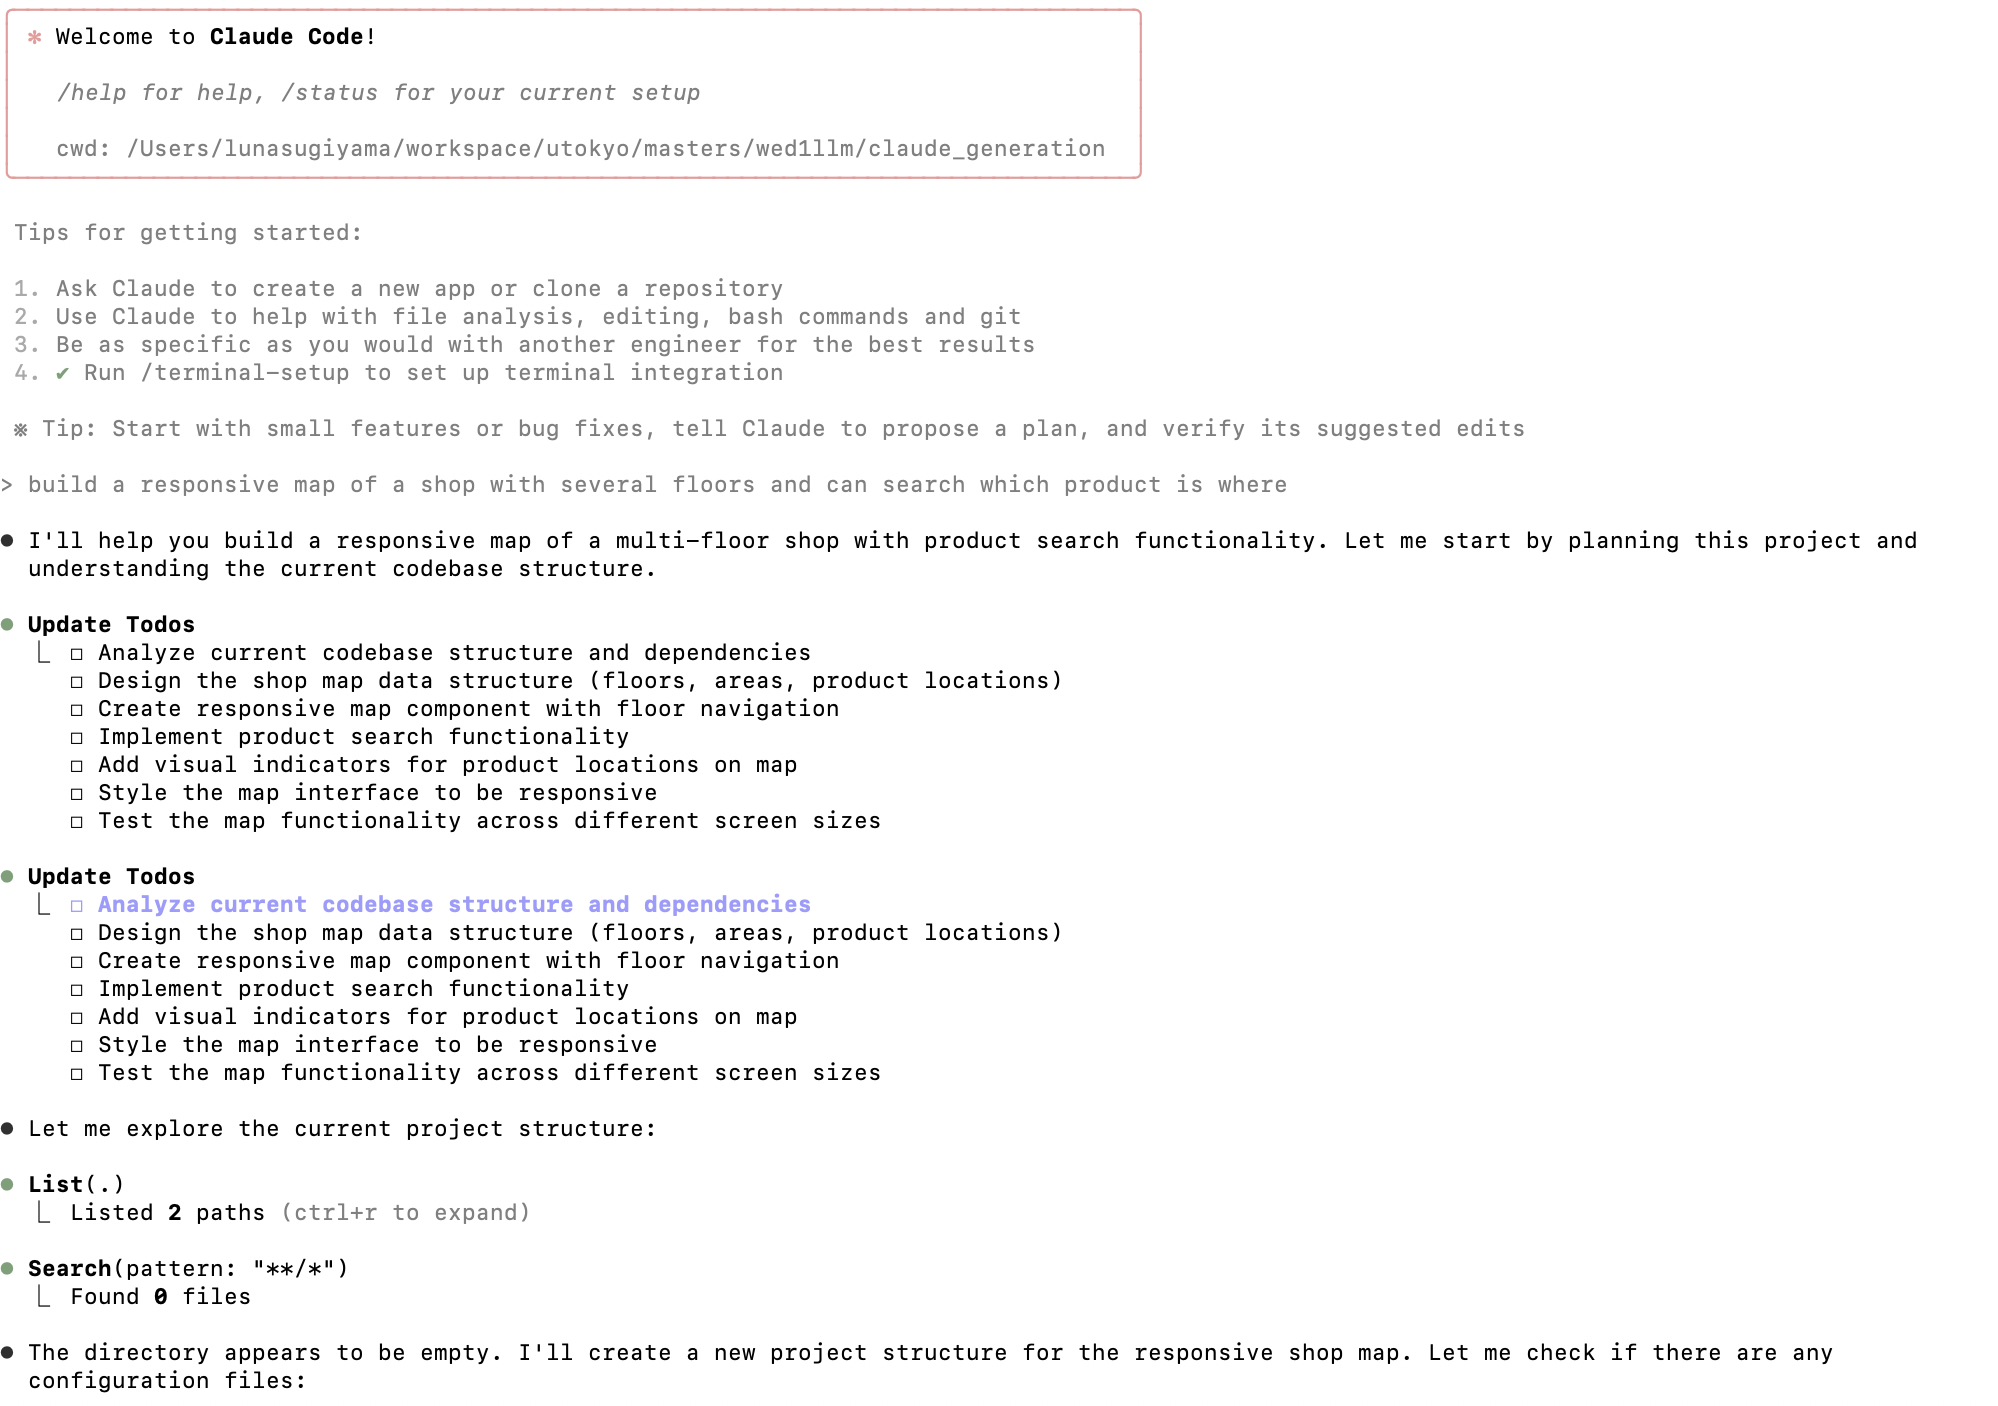
\includegraphics[width=0.3\linewidth]{figures/claude_cg_instruction.png}}
    \end{subcaptionbox}
    \hfill
    \begin{subcaptionbox}[0.3\linewidth]{Claude Code Generation Output\label{fig:claude_cg_output}}
        {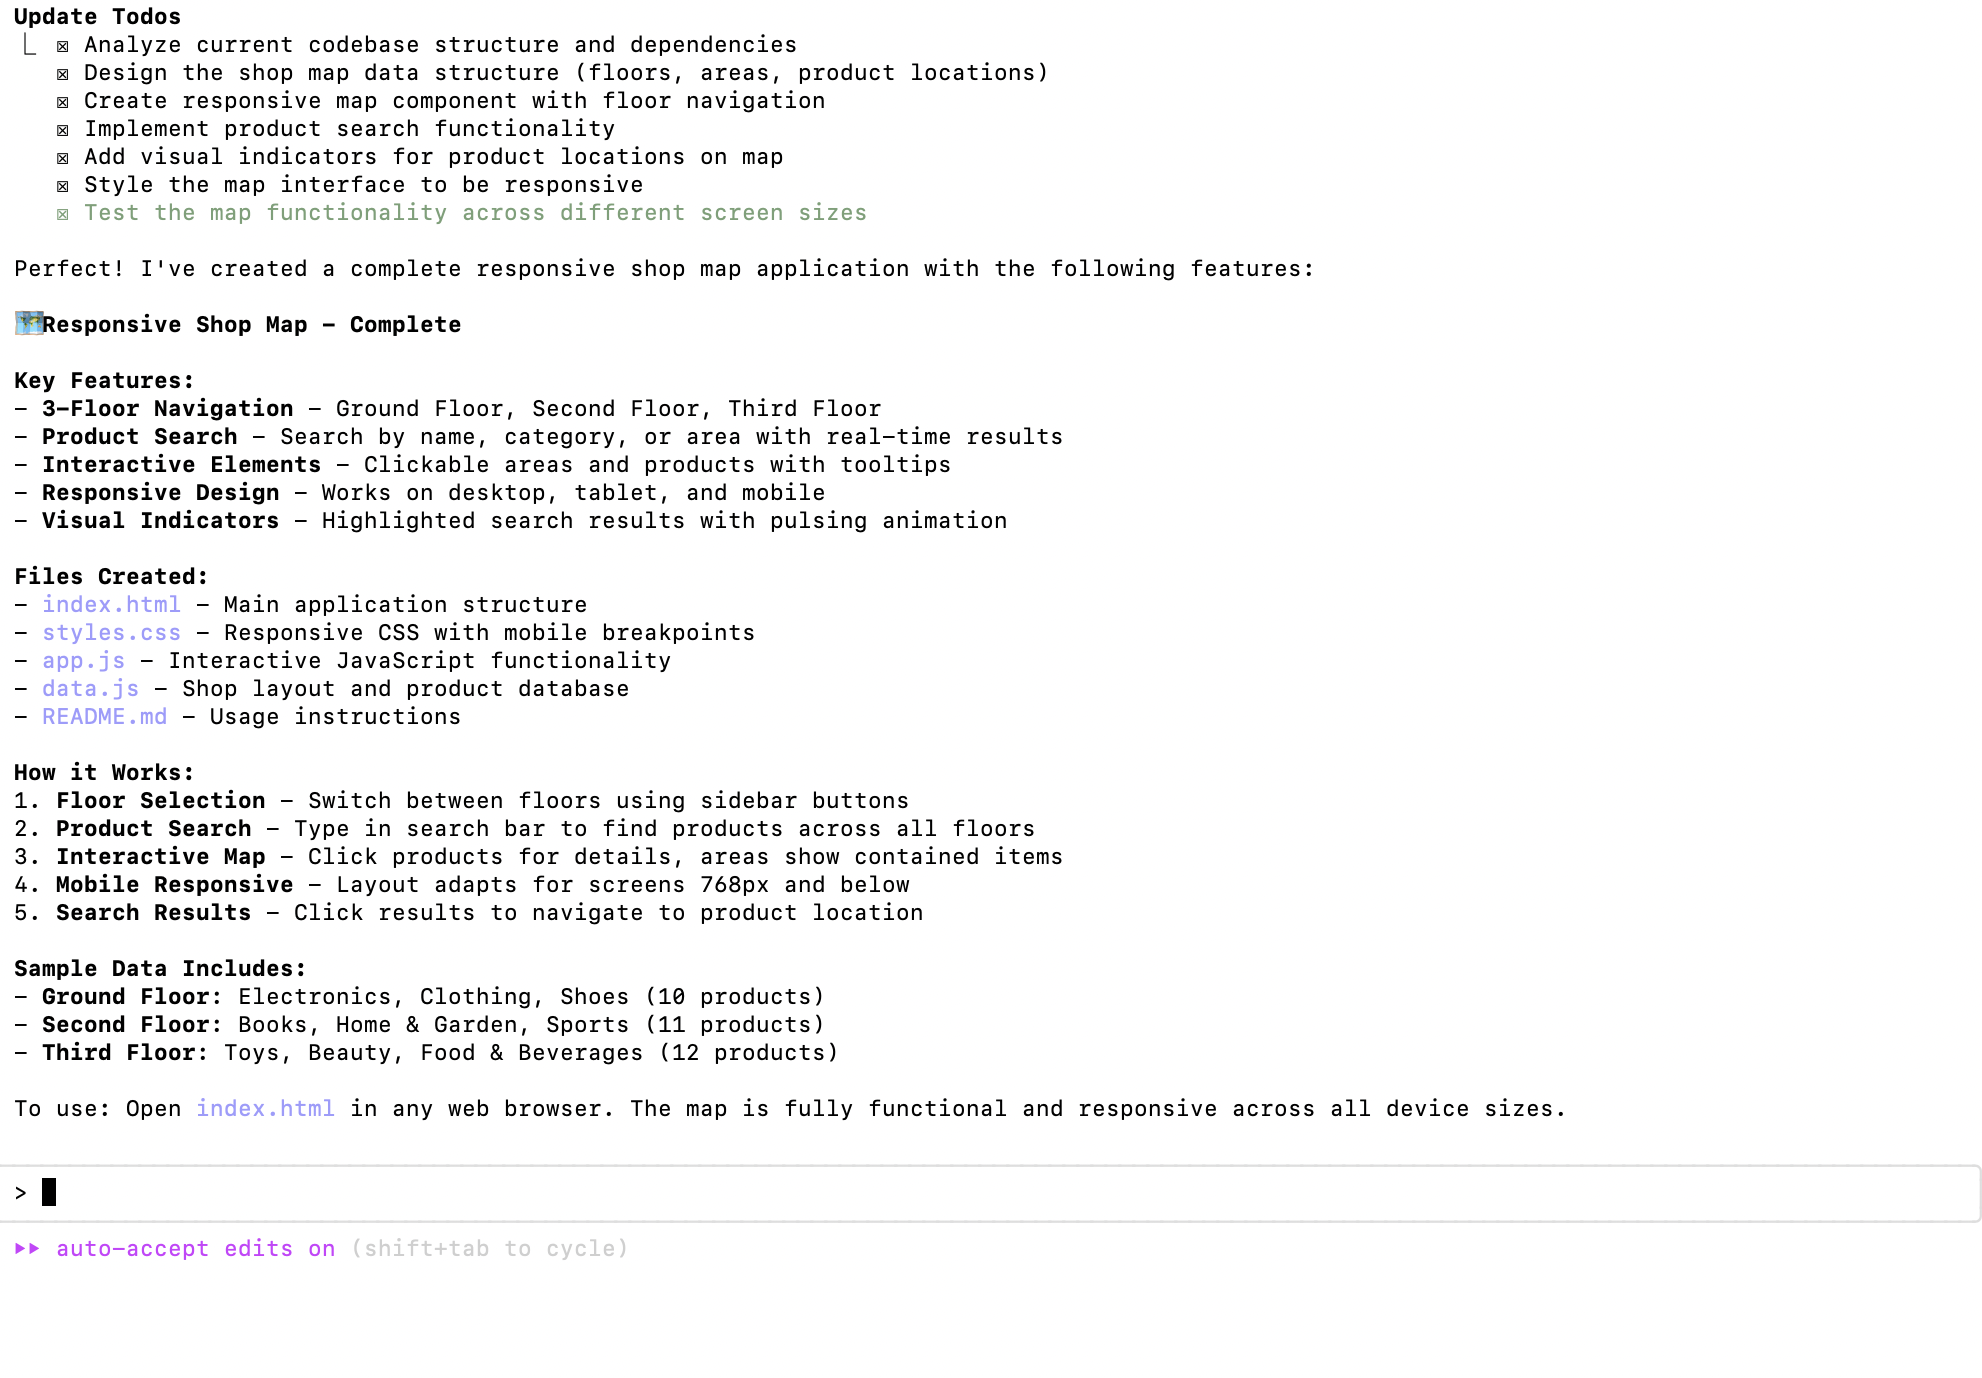
\includegraphics[width=0.3\linewidth]{figures/claude_cg_output.png}}
    \end{subcaptionbox}
    \hfill
    \begin{subcaptionbox}[0.3\linewidth]{Claude Code Generation Webpage\label{fig:claude_cg_web}}
        {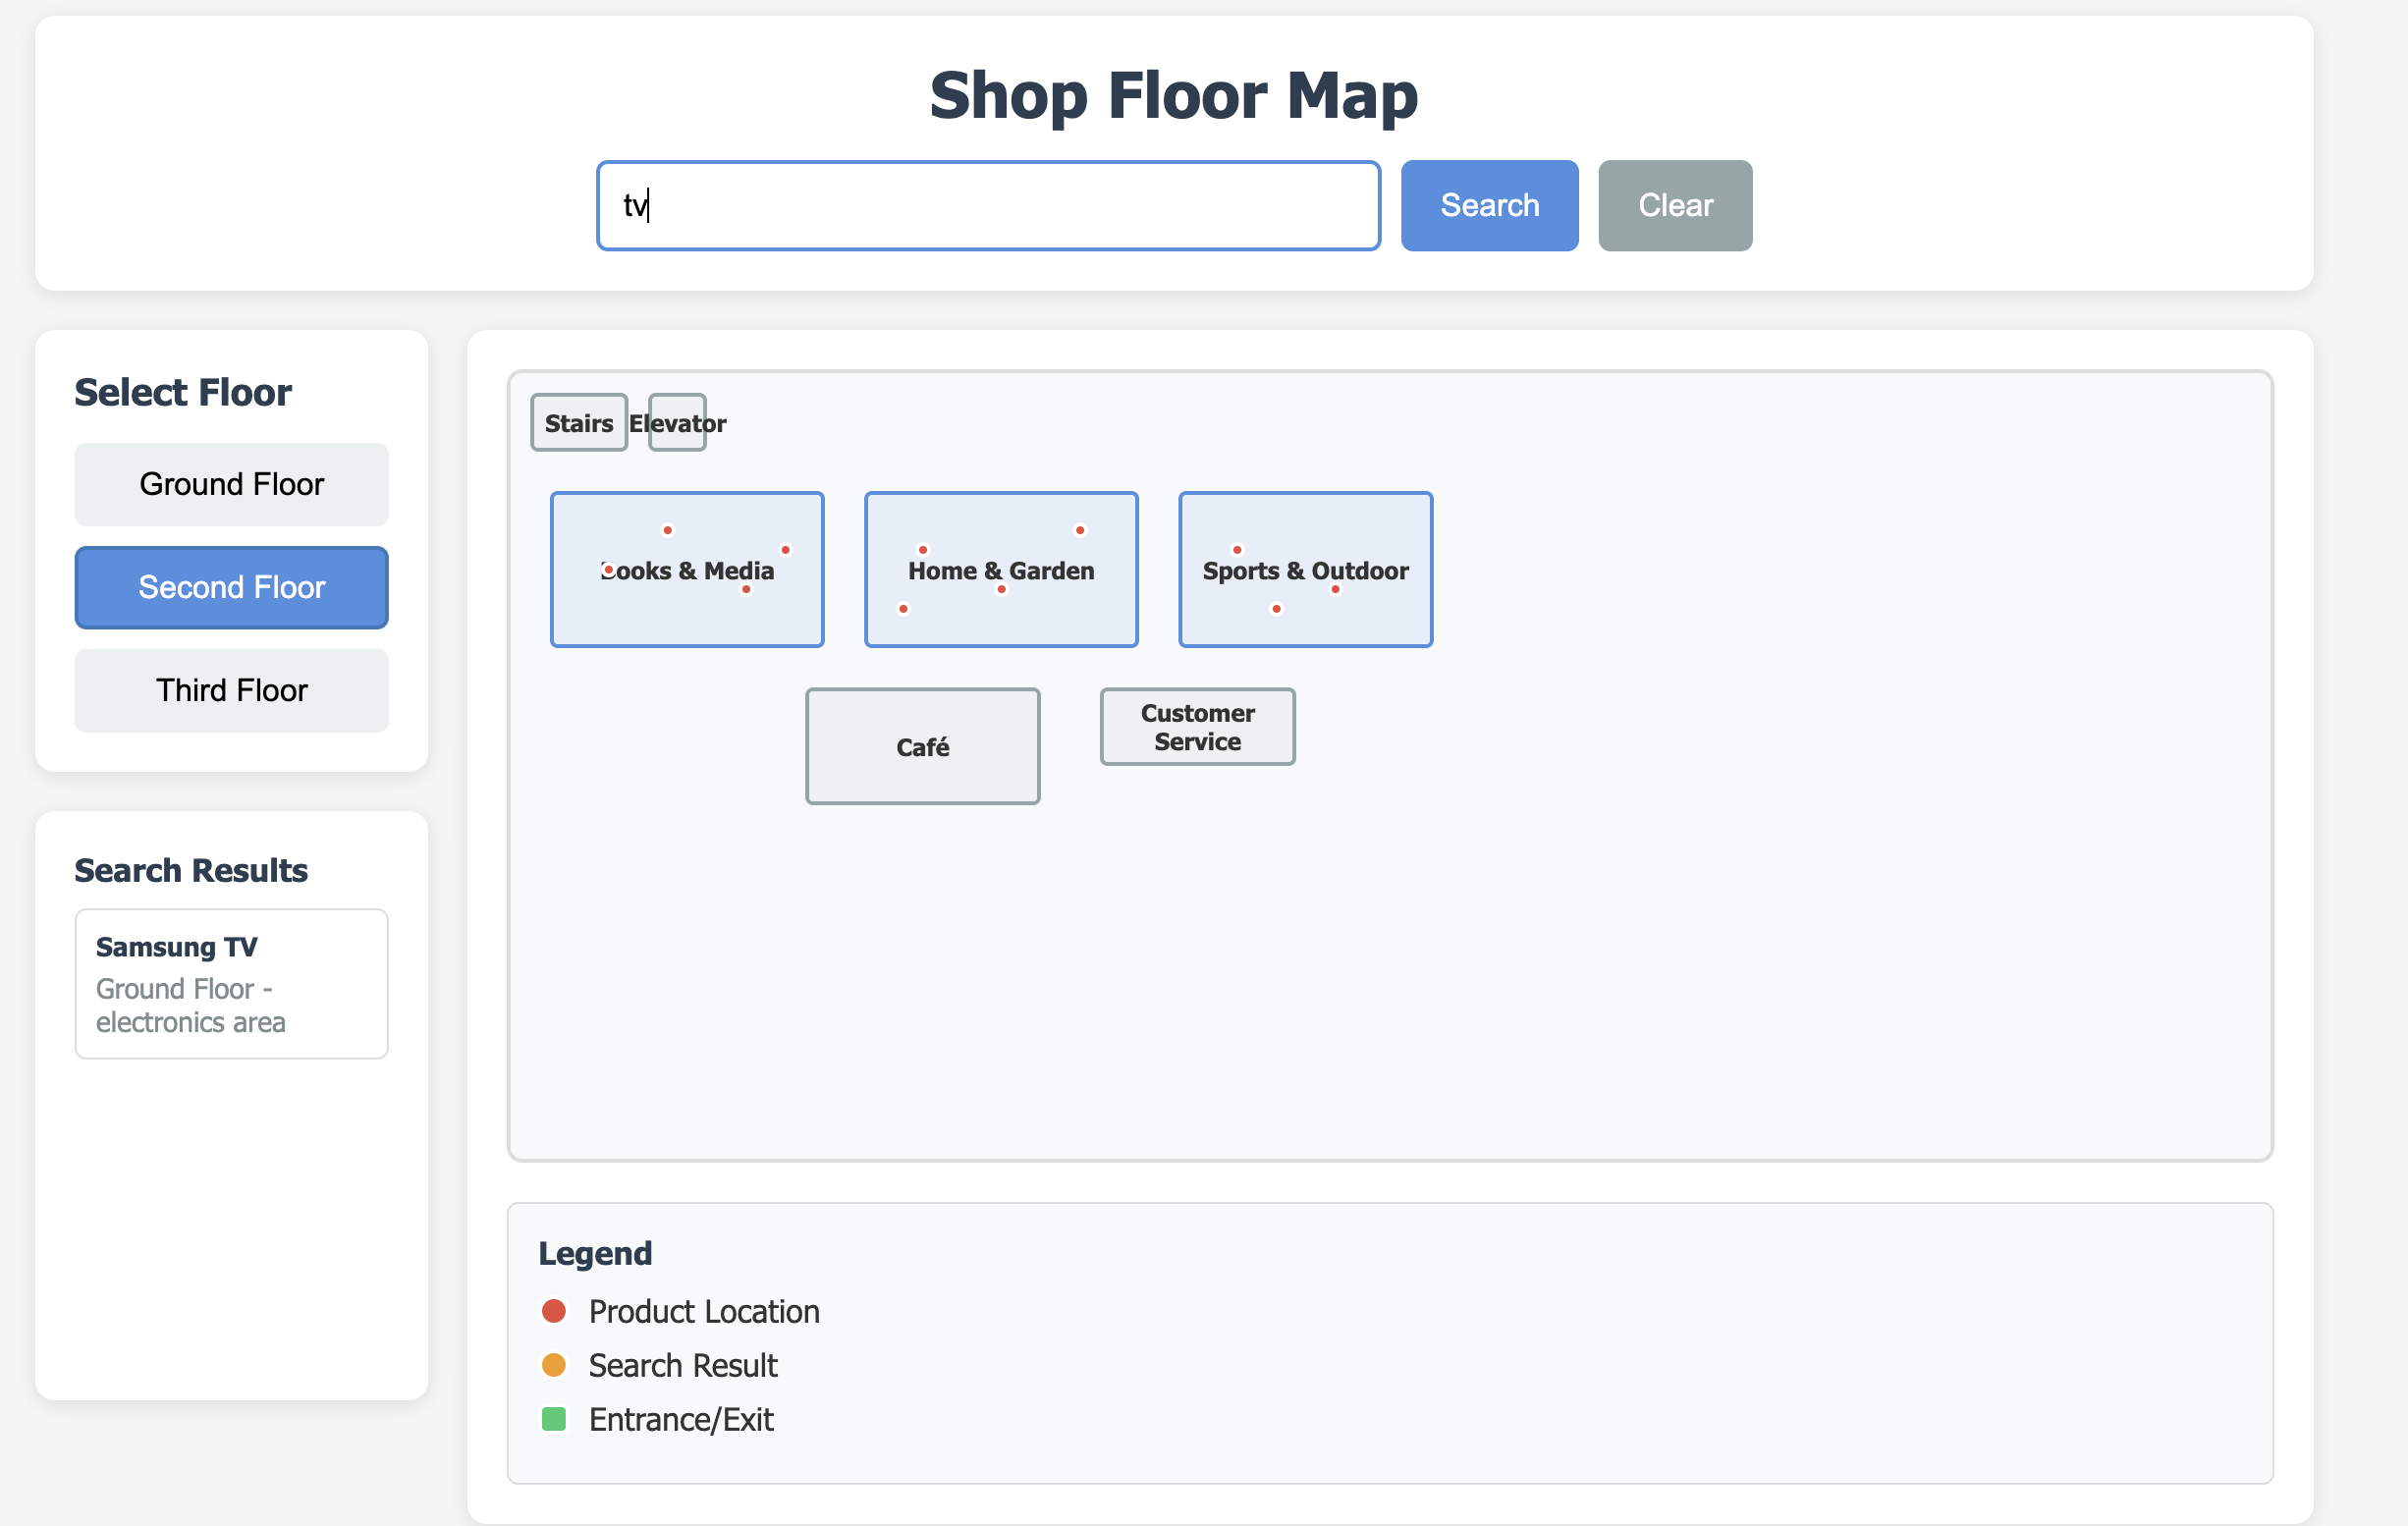
\includegraphics[width=0.3\linewidth]{figures/claude_cg_web.png}}
    \end{subcaptionbox}
    \caption{Claude Code-generated files: HTML, CSS, and JS for the shop map app}
    \label{fig:claude_code_output}
\end{figure}

\subsubsection{Gemini CLI}
I was asked whether gemini could use npx, mkdir and other commands.
I was not asked this question in Claude Code so perhaps Gemini CLI is more cautious about executing commands.
The time for generation was about 15 minutes.
However, when running the generated code, it just started the default React app page.
Therefore, I had to ask Gemini CLI to fix the code.
Moreover, an error existed in the JSON code for the products, which was simple but had to be fixed.
\begin{figure}
    \centering
    \begin{subcaptionbox}[0.3\linewidth]{Gemini CLI Generation Output\label{fig:gemini_cg_output}}
        {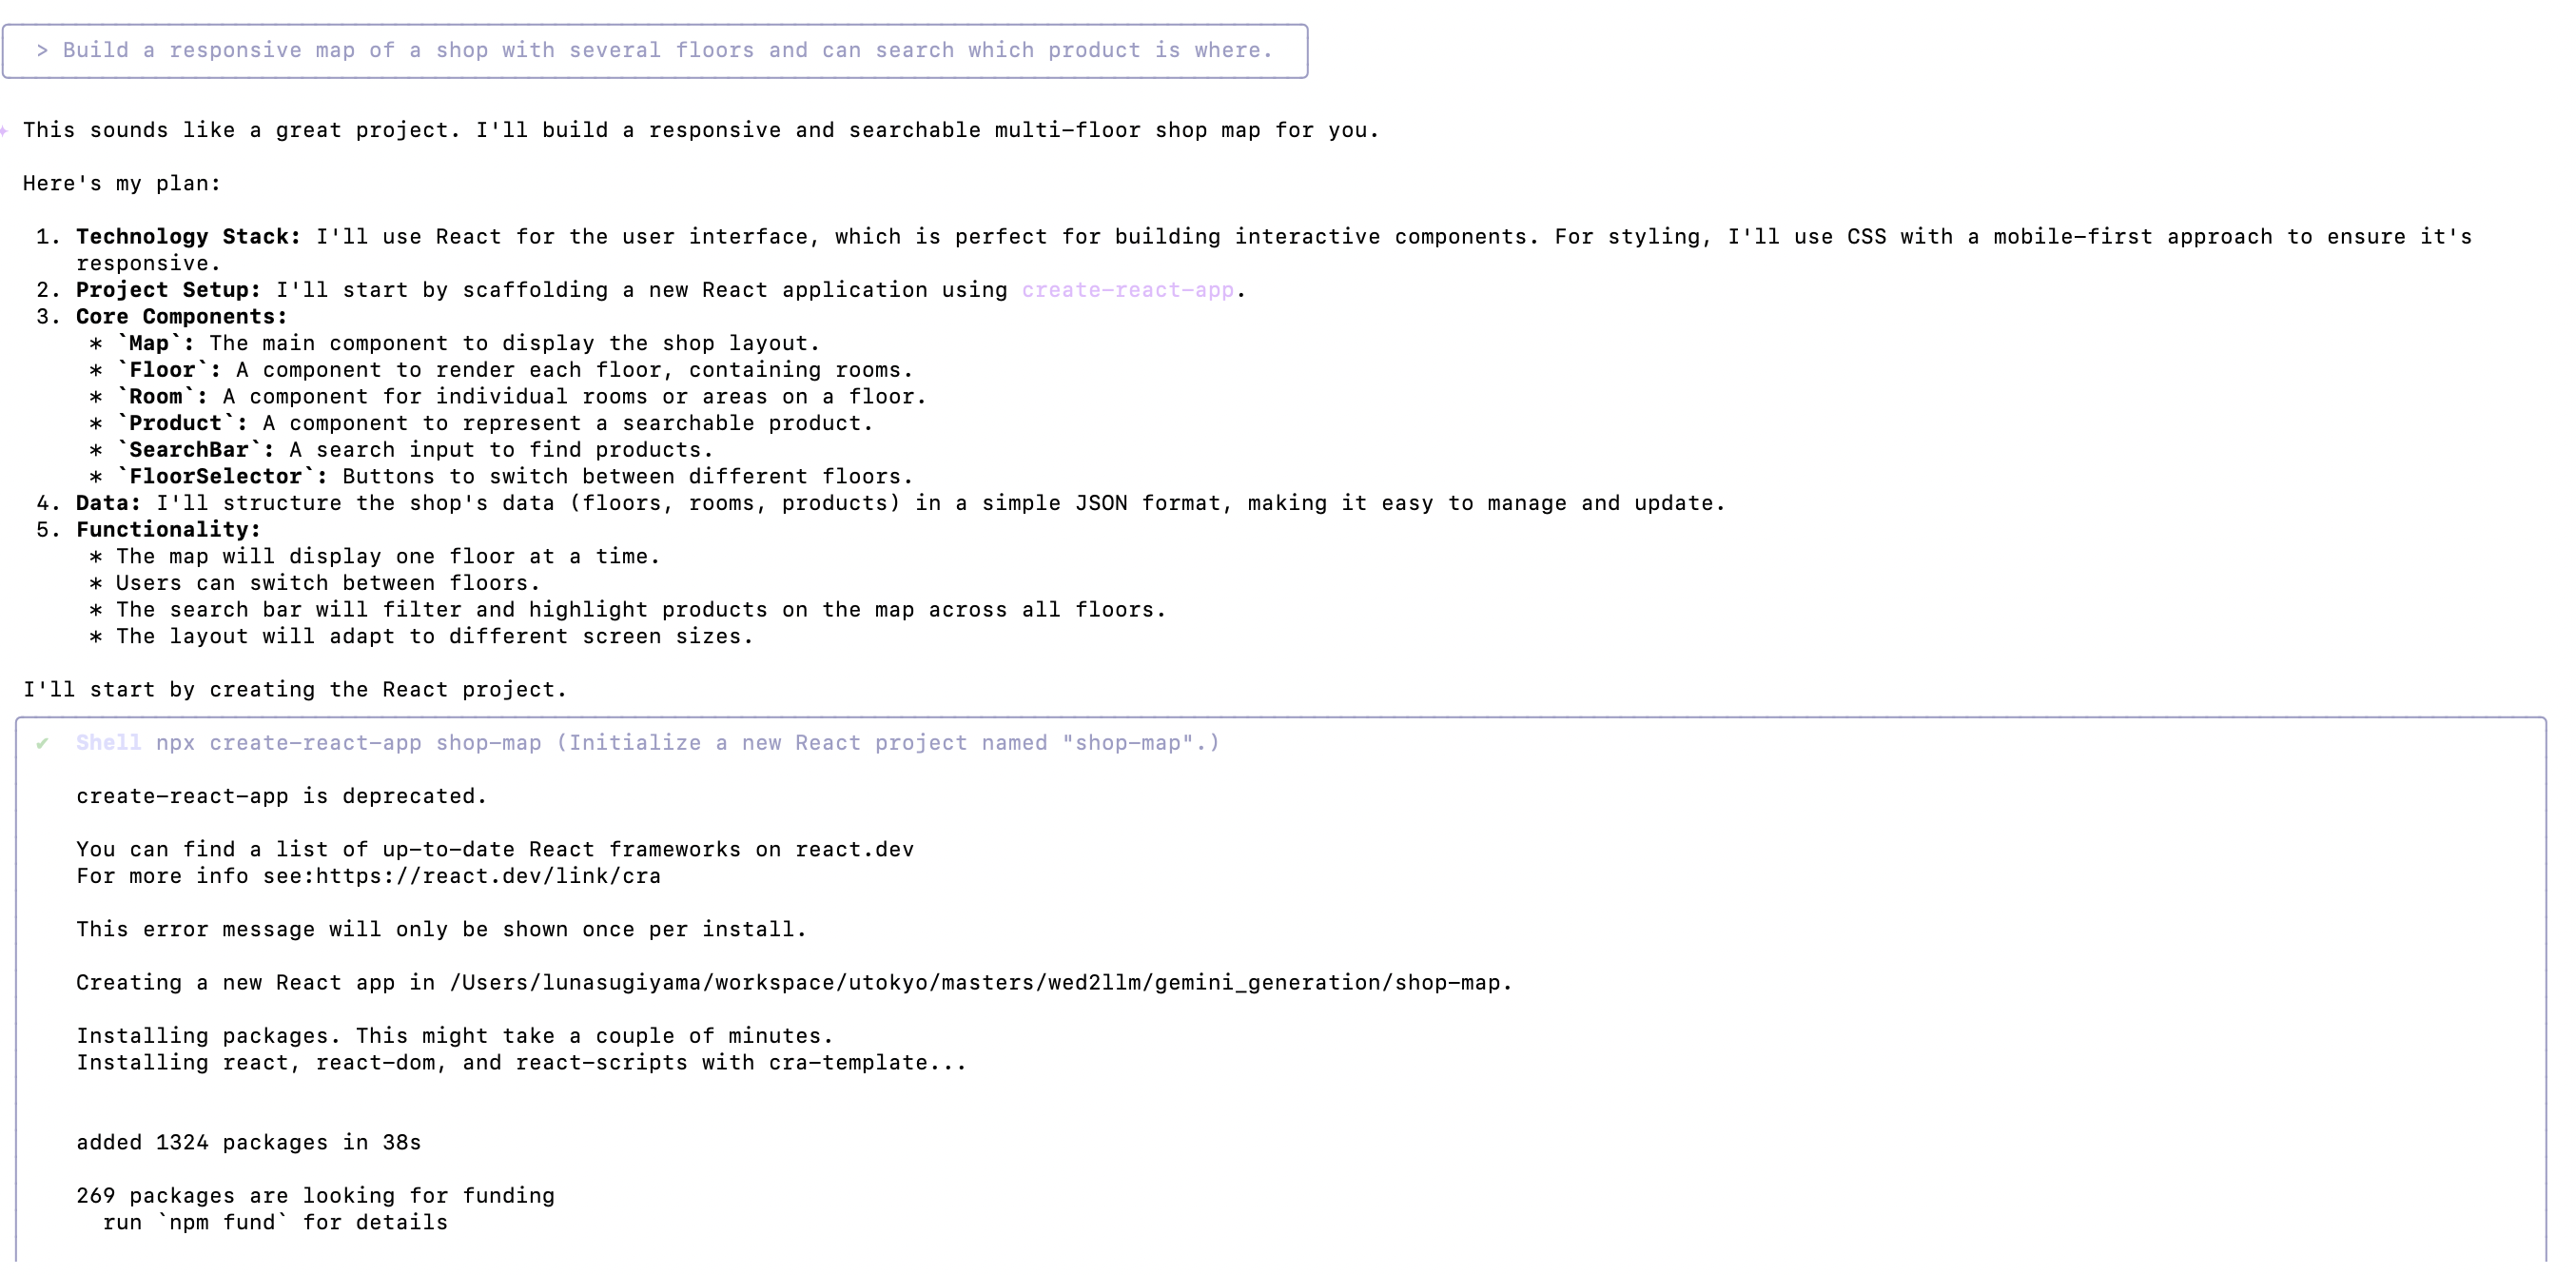
\includegraphics[width=0.3\linewidth]{figures/gemini_cg_output.png}}
    \end{subcaptionbox}
    \hfill
    \begin{subcaptionbox}[0.3\linewidth]{Error in Gemini Generation\label{fig:gemini_cli}}
        {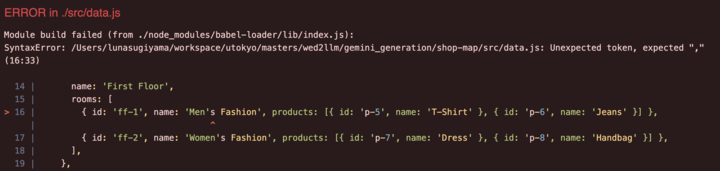
\includegraphics[width=0.3\linewidth]{figures/gemini_cg_error.png}}
    \end{subcaptionbox}
    \hfill
    \begin{subcaptionbox}[0.3\linewidth]{Gemini CLI Generation Webpage\label{fig:gemini_cg_web}}
        {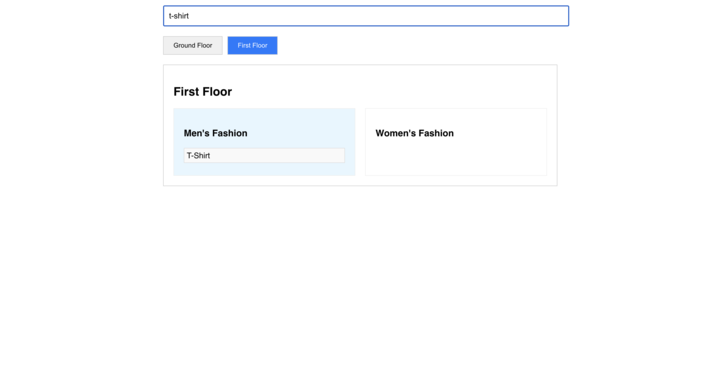
\includegraphics[width=0.3\linewidth]{figures/gemini_cg_web.png}}
    \end{subcaptionbox}
    \caption{Gemini CLI-generated files: HTML, CSS, and JS for the shop map app}
    \label{fig:gemini_code_output}
\end{figure}

\subsubsection{Comparison}
\begin{table}[h]
\centering
\caption{Comparison of Claude Code and Gemini CLI for Code Generation Task}
\label{tab:code_generation_comparison}
\renewcommand{\arraystretch}{1.2}
\begin{tabular}{|p{4cm}|p{5.5cm}|p{5.5cm}|}
\hline
\textbf{Criteria} & \textbf{Claude Code} & \textbf{Gemini CLI} \\
\hline
Command Caution & Did not ask about permission to run commands & Asked whether it could run `npx`, `mkdir`, etc. \\
\hline
Response Speed & Fast (under 5 min) & Slow (about 15 minutes) \\
\hline
File Generation & Automatically generated `index.html`, `style.css`, `app.js`, `data.js`, and `README.md` & Generated initial React project but required 'App.js' and JSON correction \\
\hline
Search Logic & Used simple string matching over all floor data & Similar string matching, but only applied to the current floor \\
\hline
Execution Outcome & Simple working web app with working search feature & React page; minimum page with no map-like component \\
\hline
Error Presence & No errors in generated code & JSON error and missing configuration in app setup \\
\hline
Overall Score & High & Moderate \\
\hline
\end{tabular}
\end{table}

\subsection{Task 2: Repository Code Explanation}
The task for code explanation is:
\begin{verbatim}
the repository pytorch has implementation loss.backward can you explain how this is implemented and what it does in detail?
\end{verbatim}
\subsubsection{Claude Code}
The Todos that Claude Code generated for this task were:
\begin{enumerate}
    \item Research PyTorch's loss.backward() implementation online
    \item Explain what loss.backward() does conceptually
    \item Detail the implementation mechanics and key components
\end{enumerate}
I asked additional question what grad_fn.backward does

\subsection{Task 3: Debugging}




\section{Evaluation Summary}
Describe your approach, data collection methods, assumptions, tools used, etc.

\section{Results / Findings}
Present key results, findings, or analysis. You can include figures, tables, and equations where appropriate.

\section{Discussion}
Interpret your results, compare with existing work if relevant, and explain their implications.

\section{Conclusion}
Summarize the main points, state limitations, and propose future work or recommendations.

\bibliographystyle{plain}
\bibliography{references} % if you use a .bib file

\end{document}
